% !TEX root = ../main.tex
\ulfgchapter{5}{Synthetic Benchmark Results}{chp:synthetic}

\section{Introduction}

This chapter reports what the protocol of Chapter~\ref{chp:detectors} returned when applied to the
benchmark of Chapter~\ref{chp:simulator}. It is a results chapter: it states what was measured, and
leaves the question of \emph{why} to Chapter~\ref{chp:attribution} and the question of whether it
generalises to Chapter~\ref{chp:realdata}.

Four measurements are reported, in the order that makes them interpretable.

\begin{enumerate}
\itemsep2pt
\item \textbf{Was the operating point actually matched?} A comparison at a supposedly common
false-alarm rate means nothing until that is verified, so it is checked first.
\item \textbf{The headline result}: detection probability per condition, with confidence intervals
and a correction for multiple comparisons.
\item \textbf{The same result in decibels}, which is the currency the comparable literature of
Section~\ref{sec:sota} reports, and which makes the margin externally interpretable.
\item \textbf{What the headline does not show}: localisation, tolerance sensitivity and
computational cost, each of which qualifies the result in a different direction.
\end{enumerate}

The frozen test split was read once, after the configuration and protocol were fixed. Every number
below comes from that single read.

\section{The operating point was matched}

Chapter~\ref{chp:detectors} argued that matching at design $\Pfa$ is not sufficient, because the
achieved rate and the design rate differ, and differ by a different amount for each variant. That
argument is only useful if the matching then worked.

Figure~\ref{fig:oppoint} shows the achieved per-cell false-alarm rate for every arm and every
condition, as a ratio to the design rate of $10^{-4}$.

\begin{figure}[H]
\centering
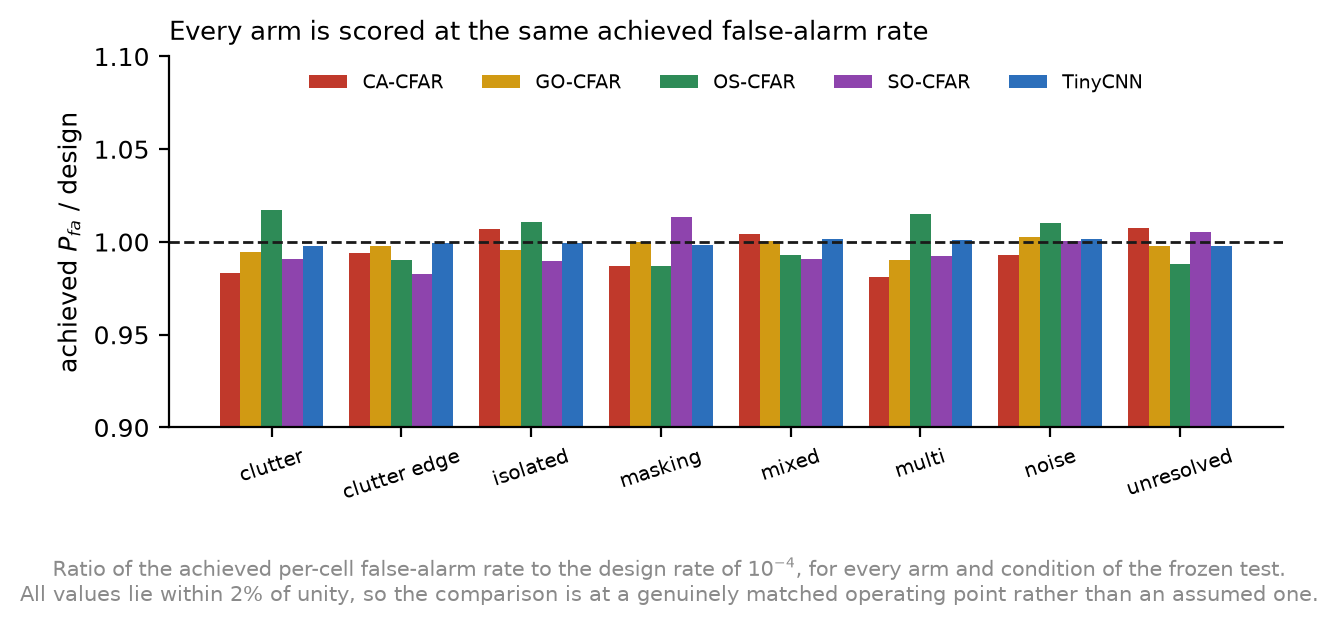
\includegraphics[width=0.92\textwidth]{figures/Chapter5/ch5_fig5_operating_point.png}
\caption[Achieved operating point]{Achieved per-cell false-alarm rate divided by the design rate,
for all five arms across all scored conditions of the frozen test split.}
\label{fig:oppoint}
\end{figure}

Every value lies between \PfaRatioMin{} and \PfaRatioMax{} --- within two per cent of unity. The
comparison that follows is therefore at a genuinely common measured operating point, not at an
assumed one.

\section{Detection probability by condition}

Figure~\ref{fig:headline} gives the headline measurement: detection probability for the frozen
network against the best CFAR variant for each condition, at the primary $\pm\ProtocolGate$-bin
gate.

\begin{figure}[H]
\centering
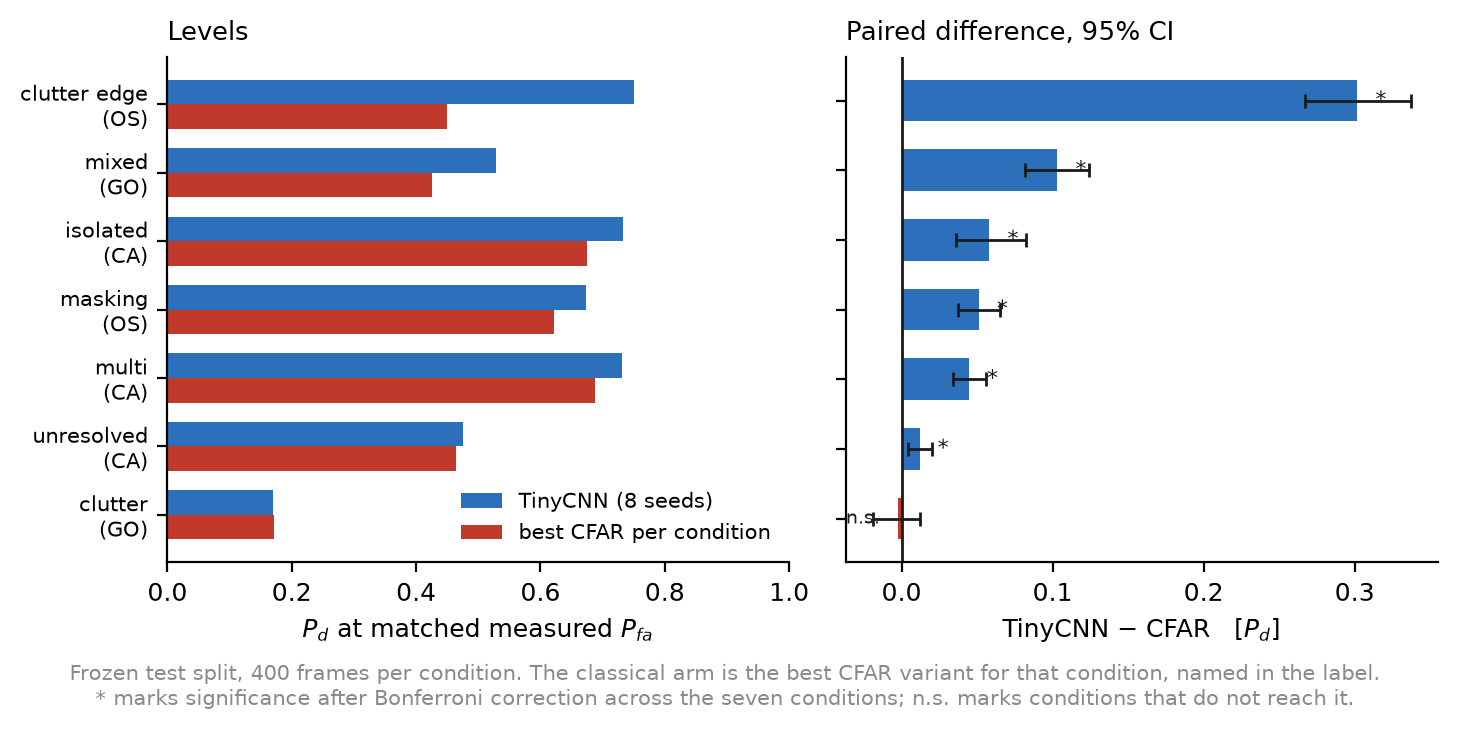
\includegraphics[width=\textwidth]{figures/Chapter5/ch5_fig1_headline.png}
\caption[Detection probability by condition]{Left: detection probability at matched measured
$\Pfa$. Right: the paired difference with its \SI{95}{\percent} bootstrap confidence interval.
The classical arm is the best-performing CFAR variant for that condition, which is a deliberately
demanding comparator.}
\label{fig:headline}
\end{figure}

Two features of the comparison deserve emphasis before the numbers.

\textbf{The classical arm is the best variant per condition.} Rather than fixing one variant
throughout, each condition is scored against whichever of CA, GO, SO or OS performs best there.
This is a stronger baseline than any single detector could achieve in deployment, because it
amounts to an oracle choosing the right variant for a condition it has already seen. The margin
reported is therefore a conservative one.

\textbf{Eight seeds, not one.} Every network value is the mean over \TinySeeds{} independently
trained seeds.

Table~\ref{tab:synresults} gives the values.

\begin{table}[H]
\centering
\caption{Detection probability at matched measured $\Pfa$ on the frozen test split, primary gate.
The CFAR column is the best variant for that condition, named in brackets.}
\label{tab:synresults}
\begin{tabular}{@{}lccc@{}}
\toprule
\textbf{Condition} & \textbf{TinyCNN} & \textbf{Best CFAR} & \textbf{Difference} \\
\midrule
Clutter edge & \SynClutterEdgeDL & \SynClutterEdgeCFAR{} (\SynClutterEdgeMethod) &
\textbf{\SynClutterEdgeDiff} \\
Mixed        & \SynMixedDL & \SynMixedCFAR{} (\SynMixedMethod) & \SynMixedDiff \\
Isolated     & \SynIsolatedDL & \SynIsolatedCFAR{} (\SynIsolatedMethod) & \SynIsolatedDiff \\
Masking      & \SynMaskingDL & \SynMaskingCFAR{} (\SynMaskingMethod) & \SynMaskingDiff \\
Multi-target & \SynMultiDL & \SynMultiCFAR{} (\SynMultiMethod) & \SynMultiDiff \\
Unresolved   & \SynUnresolvedDL & \SynUnresolvedCFAR{} (\SynUnresolvedMethod) &
\SynUnresolvedDiff \\
\midrule
Clutter      & \SynClutterDL & \SynClutterCFAR{} (\SynClutterMethod) & \SynClutterDiff{} (n.s.) \\
\bottomrule
\end{tabular}
\end{table}

The network leads in \SynWins{} of the \SynConditions{} conditions, each significant after
Bonferroni correction. The margin is far from uniform: it ranges from \SynUnresolvedDiff{} on the
unresolved stratum to \SynClutterEdgeDiff{} at clutter edges, a factor of more than twenty between
the smallest and largest.

That pattern is itself informative, and it is consistent with the failure modes of
Section~\ref{sec:cfar_failures}.

\textbf{The largest margin is where CFAR is documented to fail.} The clutter-edge condition ---
target in clean noise with the reference window reaching into the ridge --- is where the classical
threshold is set from the wrong background. The network gains \SynClutterEdgeDiff{} there.

\textbf{The smallest margin is where physics, not the detector, is the limit.} On the unresolved
stratum both arms are close to a cap neither can exceed, and the difference of
\SynUnresolvedDiff{}, although statistically significant, is of little practical consequence.

\textbf{On homogeneous clutter the two are indistinguishable.} The difference is
\SynClutterDiff{}, with a bootstrap $p$-value of \SynClutterP{} --- nowhere near the corrected
threshold. This is the one condition in which the network does not lead, and
Section~\ref{sec:tolerance} shows that it becomes more pronounced under a wider tolerance.

\section{The result in decibels}

Per-condition probabilities are hard to compare against published work, which reports margins in
decibels of signal-to-noise ratio. Figure~\ref{fig:pdsnr} expresses the same frozen result in that
currency, using the dedicated SNR-sweep split.

\begin{figure}[H]
\centering
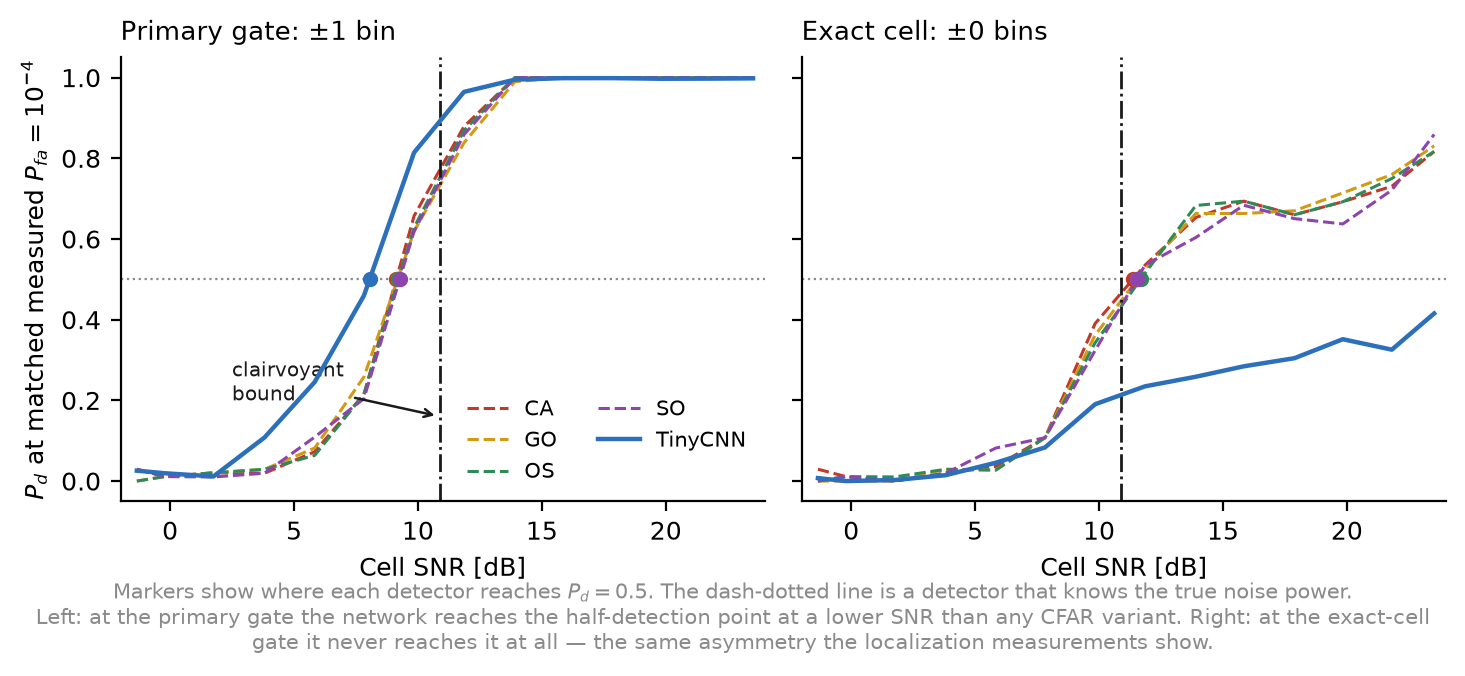
\includegraphics[width=\textwidth]{figures/Chapter5/ch5_fig2_pd_vs_snr.png}
\caption[Detection probability against cell SNR]{Detection probability as a function of measured
cell SNR at matched measured $\Pfa$. Left: the primary gate. Right: the same detectors scored on
the exact cell. The dash-dotted line marks a clairvoyant detector that knows the true noise power.}
\label{fig:pdsnr}
\end{figure}

At the primary gate the network reaches $\Pd = 0.5$ at a cell SNR of
\SI{\SynSnrFiftyDL}{\deci\bel}, against \SI{\SynSnrFiftyCA}{\deci\bel} for CA-CFAR and between
\SI{\SynSnrFiftyGO}{\deci\bel} and \SI{\SynSnrFiftySO}{\deci\bel} for the other variants. The
margin is therefore \SI{\SynSnrGainDL}{\deci\bel}: the network tolerates a target roughly
\SI{\SynSnrGainDL}{\deci\bel} weaker for the same detection rate.

The right-hand panel is the qualification, and it is a substantial one. Scored on the exact cell
rather than within one bin, the network never reaches $\Pd = 0.5$ at all, peaking at
\SynPdMaxExactDL{}, while every CFAR variant crosses it between
\SI{\SynSnrFiftyExactCA}{\deci\bel} and \SI{\SynSnrFiftyExactOS}{\deci\bel}. \textbf{The network's
advantage exists at the $\pm1$-bin gate and reverses at the exact cell.} That is a statement about
localisation rather than detection, and Section~\ref{sec:localization} measures it directly.

One further quantity is available from this figure. CA-CFAR crosses $\Pd = 0.5$ at
\SI{\SynSnrFiftyExactCA}{\deci\bel} on the exact cell, against the clairvoyant bound of
\SI{\SynSnrTheory}{\deci\bel}. The difference, \SI{\SynCfarLossCA}{\deci\bel}, is the CFAR loss of
Section~\ref{sec:cfar_loss} measured as a detection penalty --- the quantity
Section~\ref{sec:alphacal} was careful \emph{not} to conflate with the threshold-multiplier
difference. It is smaller than the \SI{\SynSnrGainDL}{\deci\bel} margin, so it cannot by itself
account for the network's advantage; Chapter~\ref{chp:attribution} takes that further.

\section{Sensitivity to matching tolerance}
\label{sec:tolerance}

Chapter~\ref{chp:detectors} committed to reporting both tolerances for every condition.
Figure~\ref{fig:tol} does so.

\begin{figure}[H]
\centering
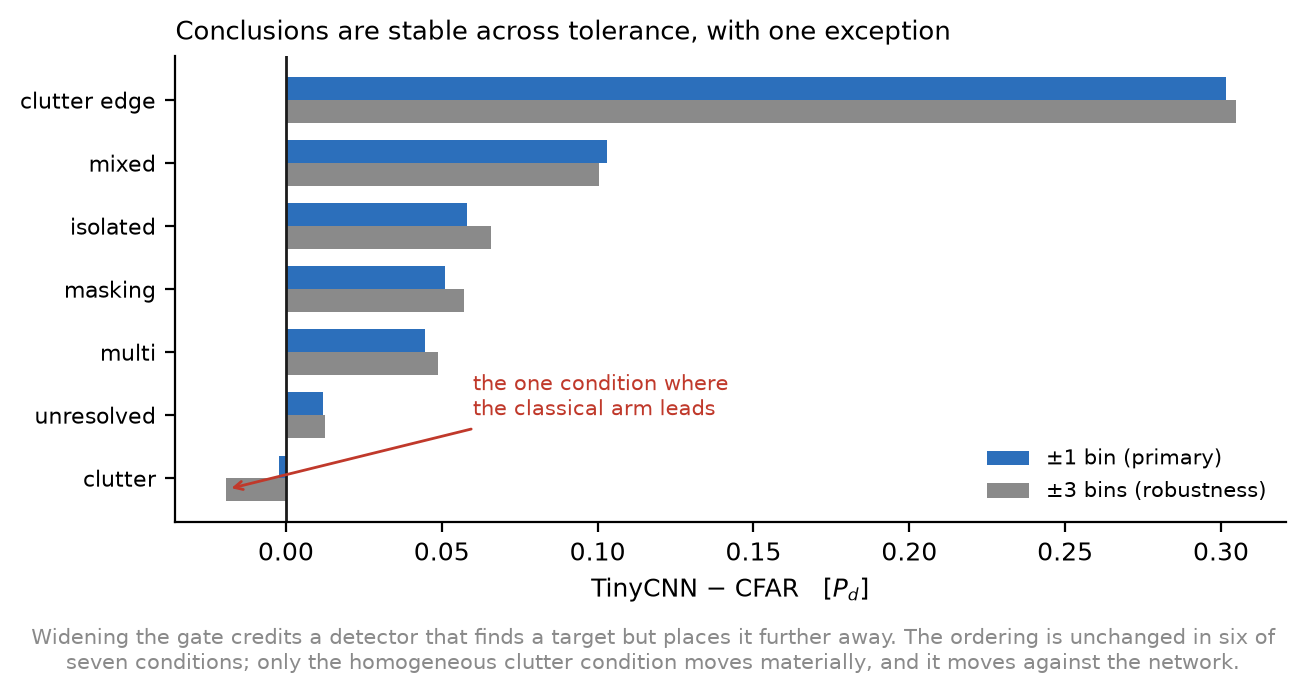
\includegraphics[width=0.92\textwidth]{figures/Chapter5/ch5_fig3_tolerance.png}
\caption[Sensitivity to matching tolerance]{The paired difference at the primary
$\pm\ProtocolGate$-bin gate and at the $\pm\ProtocolGateRobust$-bin robustness gate, for every
condition.}
\label{fig:tol}
\end{figure}

In six of the seven conditions the ordering is unchanged and the magnitude moves little. The
conclusion that the network leads on those conditions does not depend on the tolerance chosen,
which is what the robustness gate was included to establish.

The exception is homogeneous clutter. The difference there moves from \SynClutterDiff{} at the
primary gate to \SynTolThreeClutterDiff{} at the wider one. Its confidence interval is
$[\SynTolThreeClutterCIlo,\ \SynTolThreeClutterCIhi]$, and the bootstrap $p$-value is
\SynTolThreeClutterP{}. That does not reach the corrected significance threshold, so this report
does not claim the classical arm wins there.

What can be said is narrower, and still worth stating. The one condition where the network fails to
lead becomes \emph{more} pronounced when localisation precision is relaxed. That is the opposite of
what a purely detection-driven difference would do, and it is the second independent sign pointing
at localisation rather than detection.

\section{Localisation}
\label{sec:localization}

Both previous sections pointed to the same place, so it is measured directly. Localisation error is
computed over true positives only --- it asks, of the targets a detector did find, how precisely it
placed them.

\begin{figure}[H]
\centering
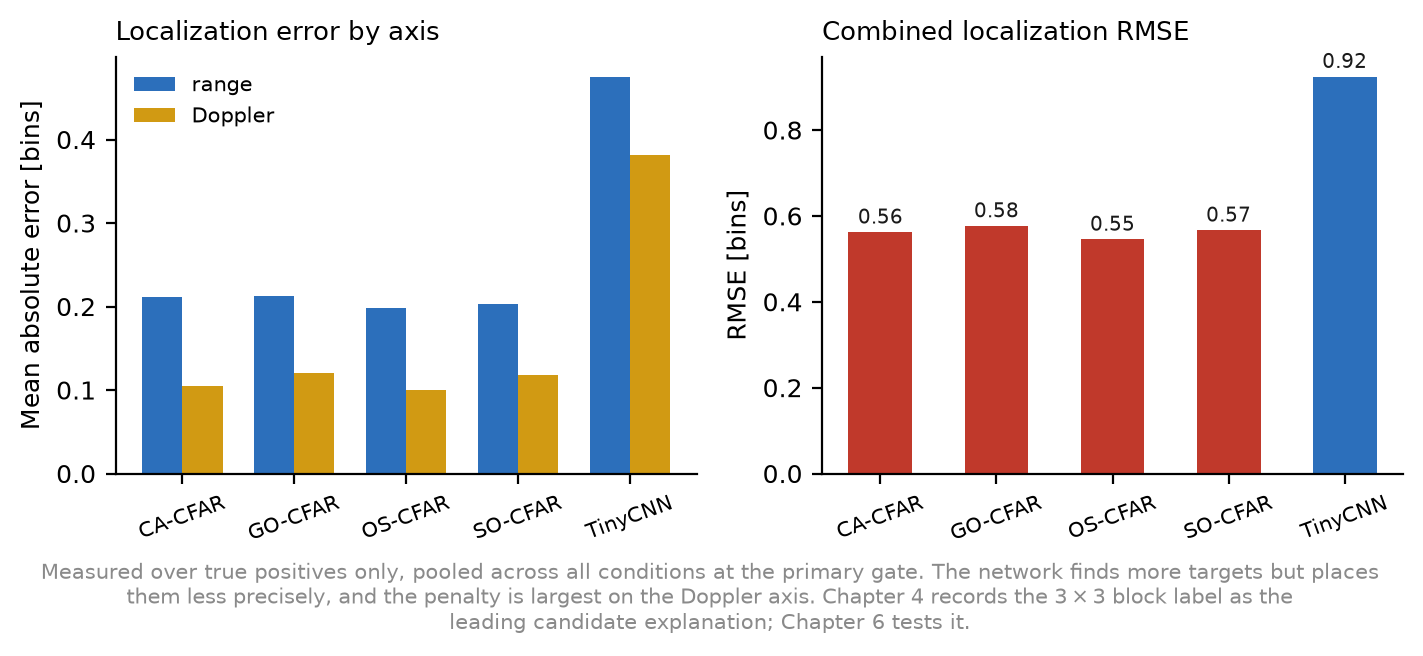
\includegraphics[width=\textwidth]{figures/Chapter5/ch5_fig4_localization.png}
\caption[Localisation error]{Mean absolute localisation error by axis, and combined RMSE, pooled
over all conditions at the primary gate. Measured over true positives only.}
\label{fig:loc}
\end{figure}

The result is unambiguous. Pooled over all conditions, the network's combined RMSE is
\LocRmseDL{} bins against \LocRmseCA{} for CA-CFAR --- \LocRmseRatio{} times worse. Broken down by
axis, the range error is \LocDrDL{} bins against \LocDrCA{}, and the Doppler error is
\LocDvDL{} bins against \LocDvCA{}, a factor of \LocDvRatio{}. In physical units the network places
detections to \SI{\LocRangeMDL}{\metre} and \SI{\LocVelMpsDL}{\metre\per\second} against CA-CFAR's
\SI{\LocRangeMCA}{\metre} and \SI{\LocVelMpsCA}{\metre\per\second}.

All four CFAR variants localise similarly well, between \LocRmseCA{} and $0.58$ bins, which
indicates that this is a property of the learned arm rather than of the evaluation.

\textbf{This is a genuine cost, and it is the counterweight to the headline result.} The network
finds more targets and places them less precisely. Which matters more depends on the application:
a tracker fed slightly imprecise but more numerous detections may do better than one fed fewer
precise ones, but that is an assertion this report has not tested.

Chapter~\ref{chp:detectors} identified the $3\times3$ block label as the leading candidate
explanation, since a block label asks the network to respond over a region rather than at one cell.
Chapter~\ref{chp:attribution} tests that explicitly rather than leaving it as a plausible story.

\section{Computational cost}

Detection probability is not the only axis on which these detectors differ.
Table~\ref{tab:runtime} gives the measured cost per frame.

\begin{table}[H]
\centering
\caption{Measured processing cost per range--Doppler frame, on the frozen test split.}
\label{tab:runtime}
\begin{tabular}{@{}lcc@{}}
\toprule
\textbf{Detector} & \textbf{Time per frame} & \textbf{Note} \\
\midrule
CA-CFAR & \SI{\RuntimeCA}{\milli\second} & cheapest; a sum per cell \\
TinyCNN & \SI{\RuntimeDL}{\milli\second} & \TinyParams{} parameters, \RuntimeMMac{} MMAC/frame \\
OS-CFAR & \SI{\RuntimeOS}{\milli\second} & a sort per cell \\
\bottomrule
\end{tabular}
\end{table}

The ordering is worth noting because it cuts both ways. The network is roughly seven times more
expensive than CA-CFAR, which is the cheapest detector here and also the one it beats by the
smallest margins on the easy conditions. But it is more than ten times \emph{cheaper} than
OS-CFAR, the variant that performs best in multi-target scenes. A learned detector is therefore not
automatically the expensive option; it is expensive relative to the simplest classical rule and
cheap relative to the most robust one.

\section{Conclusion}

On the synthetic benchmark, measured at a verified common operating point and scored through a
protocol fixed in advance:

\begin{itemize}
\itemsep3pt
\item The frozen network leads in \SynWins{} of \SynConditions{} conditions, all significant after
correction for multiple comparisons, against a per-condition best-CFAR comparator that is stronger
than any deployable single variant.
\item The margin is largest where CFAR is documented to fail --- \SynClutterEdgeDiff{} at clutter
edges --- and smallest where physics rather than the detector sets the limit.
\item Expressed in the currency the comparable literature uses, the network reaches half detection
at a cell SNR \SI{\SynSnrGainDL}{\deci\bel} lower than CA-CFAR.
\item On homogeneous clutter the two arms are statistically indistinguishable, and the difference
moves against the network when the matching tolerance is widened.
\item The network localises substantially worse: \LocRmseRatio{} times the combined RMSE of
CA-CFAR, and \LocDvRatio{} times the error on the Doppler axis. At the exact-cell gate it does not
reach half detection at all.
\end{itemize}

The headline and the qualification point in opposite directions, and both are properties of the
same frozen system. A fair one-sentence summary is that \textbf{the network detects more and places
worse}.

Two questions follow immediately, and the next two chapters take one each.
Chapter~\ref{chp:attribution} asks where the detection margin comes from and whether the
localisation penalty has the cause suspected of it. Chapter~\ref{chp:realdata} asks whether any of
this survives contact with real radar measurements.
